\begin{figure}[H]
    \centering
         \centering
         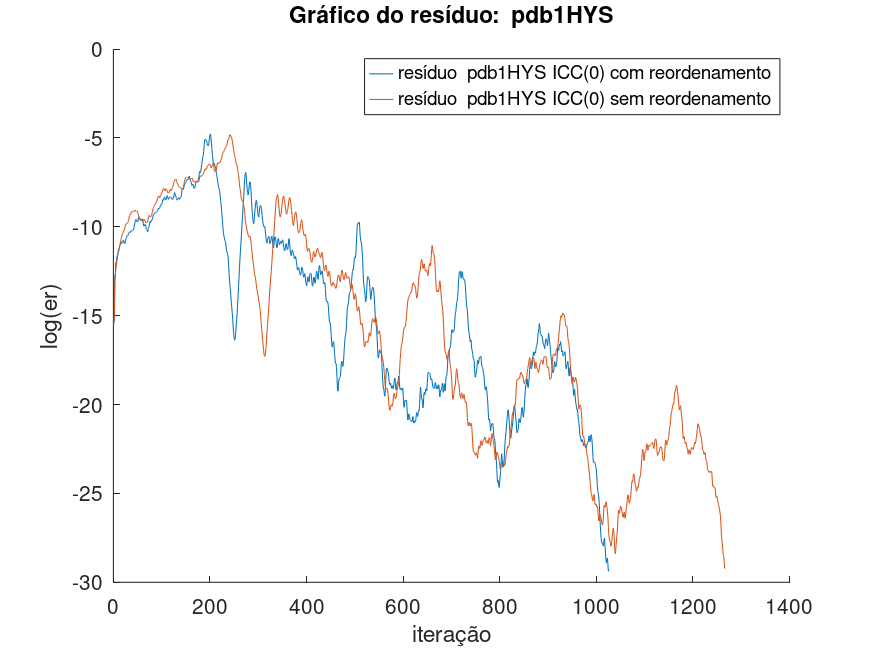
\includegraphics[width=.6\linewidth]{images/pdb1HYS.png}
         \caption{Gráfico do Resíduo da matriz \textit{pdb1HYS}}
         \label{fig:pdb-res}
\end{figure}

\begin{figure}[H]
    \centering
         \centering
         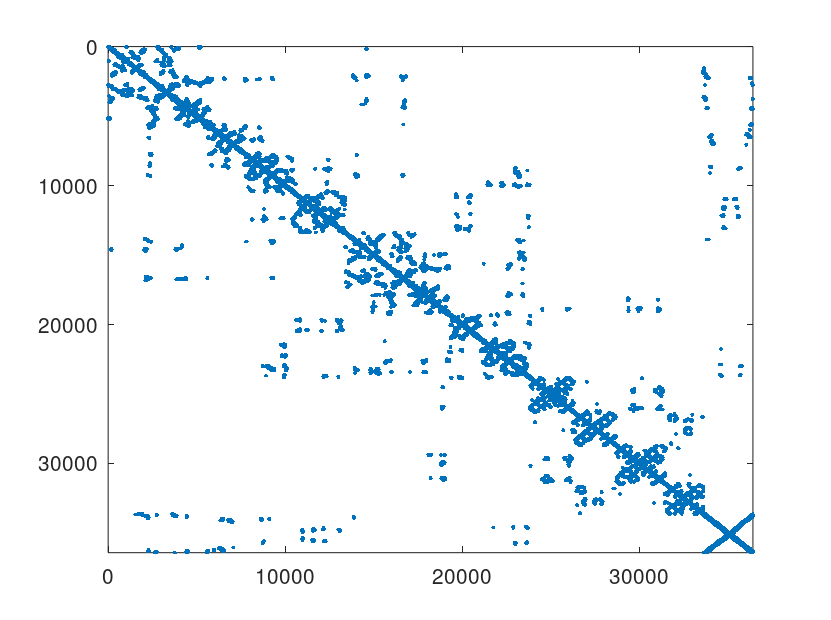
\includegraphics[width=.5\linewidth]{images/pdb1HYS_spyA.png}
         \caption{Spy de da matriz \textit{pdb1HYS}}
         \label{fig:pdb-spy-a}
\end{figure}

\begin{figure}[H]
    \centering
    \begin{subfigure}[t]{0.4\linewidth}
         \centering
         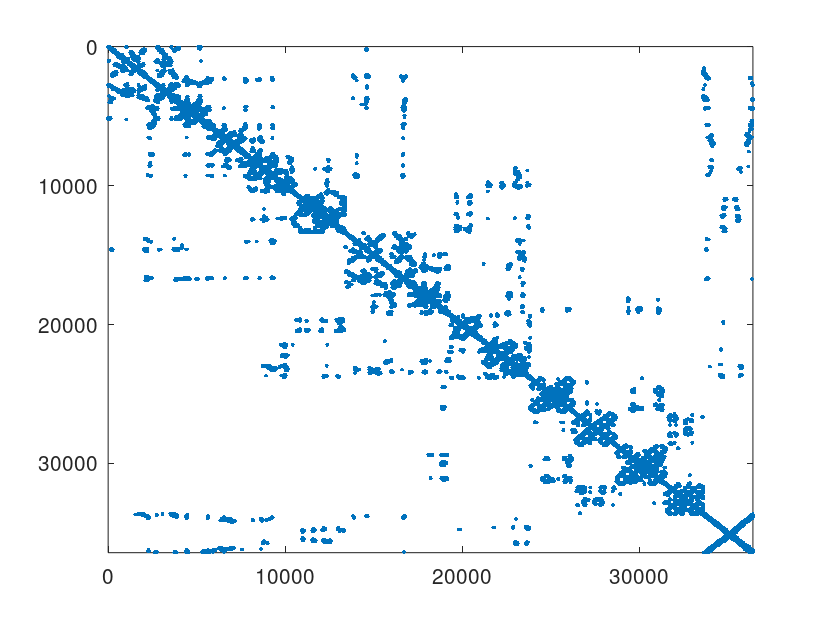
\includegraphics[width=\textwidth]{images/pdb1HYS_spyM_ICC(0)_sem.png}
         \caption{Spy após ICC(0) sem reordenamento}
         \label{fig:pdb-icc0-sem}
    \end{subfigure}
    \quad
    \begin{subfigure}[t]{0.4\linewidth}
         \centering
         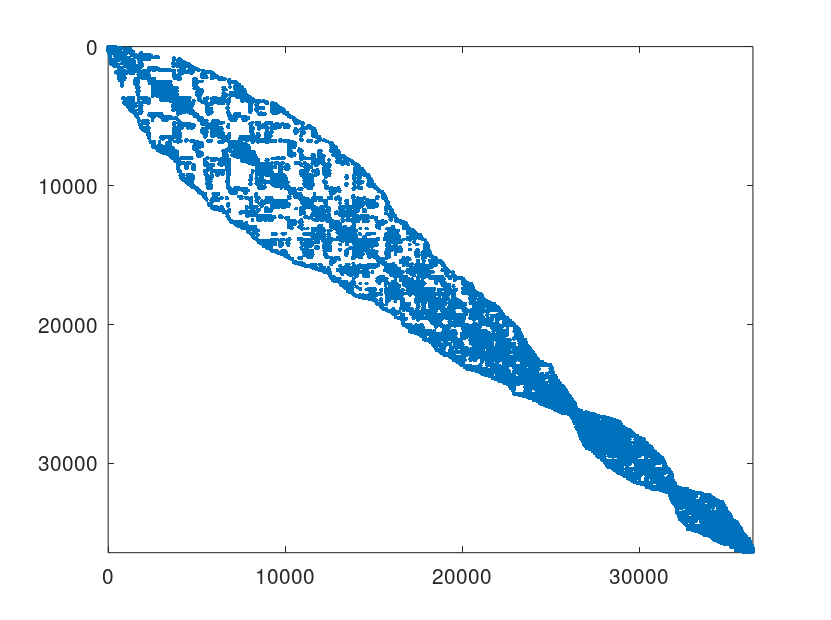
\includegraphics[width=\textwidth]{images/pdb1HYS_spyM_ICC(0)_com.png}
         \caption{Spy após ICC(0) com reordenamento}
         \label{fig:pdb-icc0-com}
    \end{subfigure}
    \label{fig:pdb}
\end{figure}